\chapter{Package structure}

The NekPy wrapper is designed to mimic the library structure of Nektar++, with
directories for the \texttt{LibUtilities}, \texttt{SpatialDomains} and \texttt{StdRegions}
libraries. This is a deliberate design decision, so that classes and definitions
in Nektar++ can be easily located inside NekPy.

There are also some other directories and files:

\begin{itemize}
	\item \path{LibUtilities/Python/NekPyConfig.hpp} is a convenience header that all 
		\texttt{.cpp} files should import. It sets appropriate namespaces for 
		\texttt{boost::python} and \texttt{boost::python::numpy}, depending on whether 
		the \texttt{Boost.NumPy} library was compiled or is included in Boost,
	\item \path{cmake/python} contains templates for \texttt{init.py} and \texttt{setup.py}
		files which every Python package should contain,
	\item \path{cmake/ThirdPartyPython.cmake} is a CMake configuration file which searches for
		\texttt{Boost.Python} and prepares \texttt{make} targets for installing NekPy.
\end{itemize}

Figure \ref{fig:package_str} shows the location of Python wrapper files within Nektar++ structure. 
Every sub-module of Nektar++ hosts an additional folder for Python files and the structure of the 
Python folder mimics the structure of the sub-module itself, as shown on the left of the figure 
with \texttt{LibUtilities} sub-module. Individual \texttt{.cpp} files, such as \texttt{Expansion.cpp} 
contain the wrappers for classes and methods from corresponding Nektar++ library files whereas 
\texttt{.cpp} files named after sub-modules (e.g. \texttt{LibUtilities.cpp}) contain 
\texttt{BOOST\_PYTHON\_MODULE} definitions which create package modules (e.g. \texttt{NekPy.LibUtilities}).

\begin{figure}[h!]
	\centering
    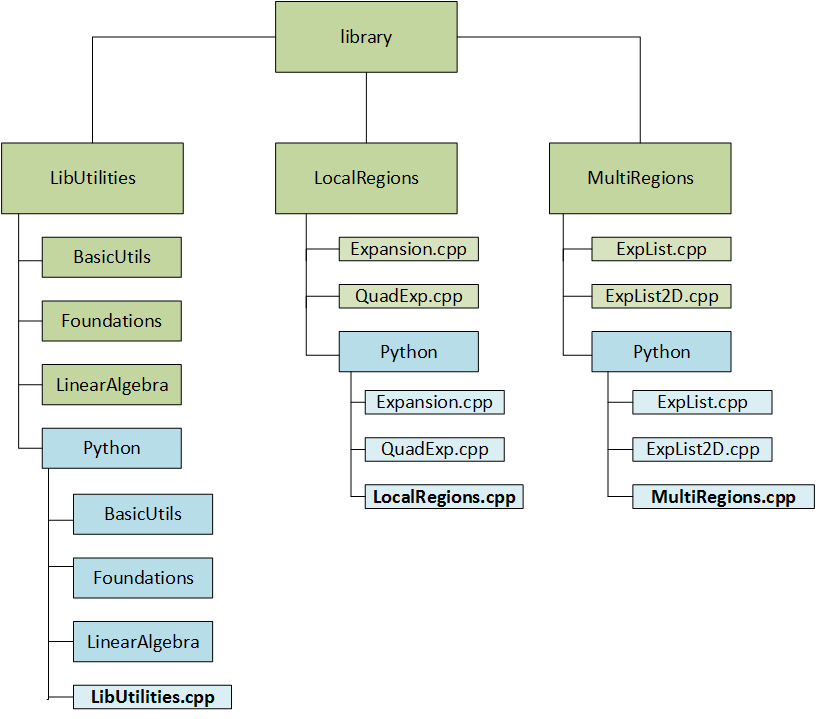
\includegraphics[width=0.9\textwidth]{img/package_str}
    \caption{The location of Python wrapper files within Nektar++ structure.}
    \label{fig:package_str}
\end{figure}